% !TEX encoding = UTF-8 Unicode
\documentclass[a4paper]{article}

\usepackage[utf8]{inputenc}
\usepackage[slovene,english]{babel}
\usepackage{sty/erk}
\usepackage{graphicx}
\usepackage[autostyle=false]{csquotes}
\usepackage[backend=biber]{biblatex}
\usepackage{listings}
\usepackage{times}
\usepackage[top=22.5mm, bottom=22.5mm, left=22.5mm, right=22.5mm]{geometry}

% Slike
\graphicspath{ {./fig/} }
% Literatura
\addbibresource{reference.bib}
% lstlisting nastavitve
\renewcommand\lstlistingname{Seznam}
\lstset{ 
    basicstyle=\footnotesize,
    captionpos=b,
    frame=single,
    keepspaces=true,
    tabsize=2,
}
% To avoid footnote on cover page:
\def\footnotemark{}


\begin{document}
\begin{sloppypar}
\title{Uporaba v mikrokrmilnik vgrajenih programirljivih logičnih vezij}

\author{Andrej Kenda, Mitja Nemec}

\affiliation{Univerza v Ljubljani, Fakulteta za elektrotehniko, Tržaška 25,
             1000 Ljubljana, Slovenija}

\email{E-pošta: andrej@kenda.one}

\maketitle



\begin{abstract}{Povzetek}
Configurable Logic Block (CLB) is a response from Texas Instruments to the
often difficult implementation of FPGA integrated circuits. This article
presents how CLB can be used in order to implement an emulation of incremental
encoder signals. In addition to presentation how the emulation is designed, the
paper discusses how the CLB behaves in practice and what are the experiences
using the tooling to program the CLB.

\end{abstract}

\selectlanguage{slovene}


\section{Uvod}
V prejšnjem članku smo pregledali zgradbo in delovanje sistema CLB (angl.
configurable logic block), ki je odgovor proizvajalca Texas Instruments na
številne težave pri implementaciji FPGA (angl. field-programable gate array). 

Kot je bilo opisano v prejšnjem članku, za programiranje omenjenega
koprocesorja uporabljamo orodje ``CLB Tool''. To nam preko grafičnega vmesnika
omogoča nastavljanje različnih podsklopov ter generira kodo za uporabo v
programu. Poleg generirane kode pa nam omogoča vpogled v vse podsklope preko
simulacijskih datotek ter dodatnega diagrama povezav.

Primer praktične uporabe CLB koprocesorja je emulacija inkrementalnega
dajalnika. Emulacija inkrementalnega dajalnika je uporabna predvsem v HIL in
PHIL sistemih \cite{lauss} \cite{nibert}, kateri so v zadnjem času vedno bolj
pogosto v uporabi za preizkušanje elektronike namenjene za krmiljenje oziroma
regulacijo električnih strojev.


\section{Idejna zasnova}
Inkrementalni dajalnik je senzor kota gredi, ki generira dva digitalna signala
A, B.  Signala sta pravokotne oblike z vklopnim razmerjem 50\% in sta med seboj
zamaknjena za 90°. Tako preko faznega premika med njima sklepamo o smeri
vrtenja, frekvenca signalov pa nosi informacijo o hitrosti vrtenja.

Za emulacijo inkrementalnega dajalnika bomo za podatek o hitrosti vrtenja
vzeli vhodni pravokotni signal, kateremu lahko spreminjamo frekvenco in ga
generiramo s ustrezno periferno enoto, ki omogoča generiranje takih signalov
(PWM števec).

V CLB koprocesorju se vhodni signal uporabi kot vir takta in iz njega izpelje
dva izhodna signala, ki sta drug drugemu zamaknjena za 90°. Poleg
tega pa je potrebno dodati tudi sposobnost za spremembo smeri ``vrtenja'', kar
pomeni da ob določenih pogojih začne ``prehitevati'' prej počasnejši signal.

Cilnji potek signalov simuliranega inkrementalnega dajalnika je prikazan na
sliki \ref{fig:enkoder_zasnova}, kjer lahko opazimo da je na vhod CLB
koprocesorja priključen kvadratni signal z vklopnim razmerjem 50\%.

Kot je to dejstvo na veliko področjih, je tudi tu možnih več
pristopov. Tako implementacija, opisana v nadaljevanju ni bila očitna že od
samega začetka in tudi samo raziskovanje je vključevalo nemalo neuspelih
poskusov.

\begin{figure}[htb]
    \centerline{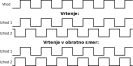
\includegraphics[width=8cm]{enkoder_zasnova}}
    \caption{Cilnji potek signalov simuliranega inkrementalnega dajalnika z
             uporabo CLB koprocesorja}
    \label{fig:enkoder_zasnova} 
\end{figure} 


\section{Nastavljanje CLB podkslopov}\label{sec:nastavitve_podsklopov}
Nastavljanje CLB enote je najlažje preko uporabe orodja ``CLB Tool''. Le-to
orodje generira ustrezne ``C'' datoteke, ki jih vključimo v projekt s katerimi
potem glavno jedro MCU-ja ustrezno nastavi CLB enoto. 

V kolikor pa želimo CLB enoto vključiti v že narejen projekt, ki temelji na
drugačni arhitekturi programske opreme, ki ne podpira uporabe ``CLB Tool''
orodja lahko omenjene datoteke generiramo tudi s spletnim orodjem
``SysConfig'', ki vsebuje povsem enak vmesnik \cite{sysconfig}.

\subsection{Splošne nastavitve}
Ker je v našem primeru CLB enota uporabljana relativno samostojno je pri
razvoju programa za CLB za preverjanje, ali je CLB enota pravilno nastavljena,
najlažje uporabiti simulacijo.  V ta namen je v orodju ``CLB Tool'' za modul
``BOUNDARY'', ki določa vhode v CLB modul, na voljo možnost izbire simuliranega
kvadratnega signala. Za implementacijo inkrementalnega dajalnika je kot
simuliran vhod definiran vhod ``in2'', kar prikazuje tudi slika
\ref{fig:clbtool_boundary}.

\begin{figure}[htb]
    \centerline{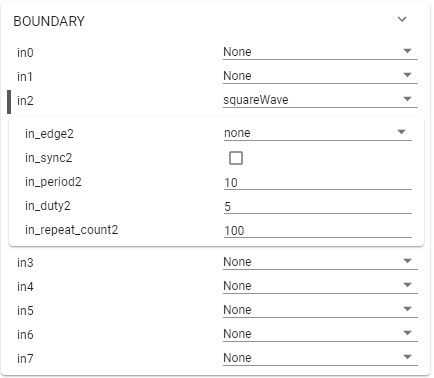
\includegraphics[width=8cm]{clbtool_boundary}}
    \caption{Konfiguracija modula ``BOUNDARY'' v orodju ``CLB Tool''}
    \label{fig:clbtool_boundary} 
\end{figure} 

\subsection{Nastavljanje parametrov}\label{sec:nastavljanje_clb}
Emulacijo inkrementalnega dajalnika smo implementirali na naslednji način:
\begin{itemize}
    \item Za vir ure/hitrosti smo uporabili eCAP modul v funkciji PWM
        generatorja s katerim smo generirali 50\% PWM signal, ki mu lahko
        nastavljamo frekvenco.
    \item Preko števca 0 in HLC-ja temu urinemu signalu prepolovimo frekvenco.
    \item Preko števca 1 in HLC-ja generiramo fazno zamaknjen signal s
        prepolovljeno frekvenco. Dodatno lahko ta signal invertiramo.
\end{itemize}

Zasnova inkrementalnega dajalnika je prikazana na sliki
\ref{fig:dobra_zasnova_shema} in uporablja 1 LUT4 modul, 2 števca in HLC modul.
Implemetirana je v naslednjih korakih, ki se navezujejo na poteke signalov s
slike \ref{fig:dobra_zasnova_shema} in \ref{fig:dobra_zasnova_potek}.
\begin{itemize}
    \item Vhod ``in2'' je direktno in negirano preko LUT4 modula speljan v
        vhoda ``e0'' in ``e1'' HLC modula (vhoda za proženje dogodkov).
    \item V HLC modulu se dogodki prožijo ob pozitivnem robu prožilnega
        signala, torej se pripadajoč dogodek sproži na vsako periodo signala
        ``in2'' (s 180° zamikom).
    \item HLC modul operira z vrednostmi ``R0'', ``R1'', ``C0'' in ``C1'', pri
        tem je začetna vrednost ``R0'' nastavljena na 1.
    \item Oba števca sta nastavljena, da ne štejeta, nimata vhodnih signalov,
        le vrednost ``MATCH1'' je nastavljena na 1 - uporabljena sta le kot
        komparatorja.
    \item Ob dogodku ``e0'' HLC modul zamenja vrednosti ``C0'' in ``R0'', pri
        tem se izvršijo naslednji ukazi:
    \begin{itemize}
        \item \textbf{MOV C0, R1} - premakni vrednost C0 v R1,
        \item \textbf{MOV R0, C0} - premakni vrednost R0 v C0,
        \item \textbf{MOV R1, R0} - premakni vrednost R1 v R0,
    \end{itemize}
    \item Pri tem se ob vsakem pozitivnem robu vhodnega signala ``e0'' zamenja
        polariteta izhodnega signala ``MATCH1'', števca 0 - perioda signala je
        dvakrat večja od vhodnega.
    \item Ob dogodku ``e1'', ki se izvrši s 180° zamikom glede na ``e0'', se v
        števec 1 vpiše vrednost števca 0 - ``MATCH1'' števca 1 je tako enak
        signalu ``MATCH1'' števca 0, le da je zakasnjen za četrtino njegove
        periode. Pri tem se izvrši ukaz:
    \begin{itemize}
        \item \textbf{MOV C0, C1} - premakni vrednost C0 v R1,
    \end{itemize}
    \item Signala ``MATCH1'' obeh števcev sta speljana na izhod.
\end{itemize}

\begin{figure}[htb]
    \centerline{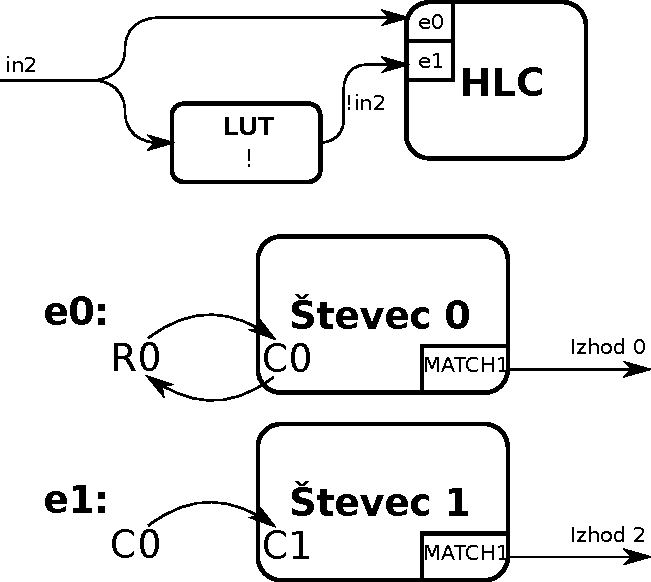
\includegraphics[width=5.5cm]{dobra_zasnova_shema}}
    \caption{Shema boljše zasnove inkrementalnega dajalnika s pomočjo CLB
             koprocesorja}
    \label{fig:dobra_zasnova_shema}
\end{figure}

\begin{figure}[htb]
    \centerline{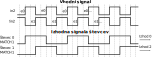
\includegraphics[width=8cm]{dobra_zasnova_potek}}
    \caption{Potek signalov boljše zasnove inkrementalnega dajalnika s slike
             \ref{fig:dobra_zasnova_shema}}
    \label{fig:dobra_zasnova_potek}
\end{figure}

\subsection{Obračanje smeri inkrementalnega dajalnika}
V drugem primeru iz poglavja \ref{sec:nastavljanje_clb} smo parametre nastavili
tako, da je signal ``MATCH1'' iz števca 1 vedno zakasnjen glede na signal
``MATCH1'' iz števca 0. Zato je potrebno dodati tudi logiko za obračanje smeri
simuliranega inkrementalnega dajalnika, saj želimo simulacijo obeh smeri
vrtenja. Za to uporabimo dodaten vhod ``in0'' v ``BOUNDARY'' modulu. Tega prav
tako nastavimo na simuliran kvadraten signal, le da mu periodo občutno povečamo
(pribl. 10-kratnik periode signala ``in2'').

Simulirani signal obravnavamo kot zunanjo tipko, ki v normalnem stanju zavzema
logično 1, ob pritisku pa logično 0. To uporabimo pri izhodu iz CLB
koprocesorja, kjer je signal potrebno speljati preko izhodnega LUT3 modula;
\begin{itemize}
    \item Signal ``MATCH1'' števca 0 je speljan preko izhodnega LUT3 modula 0,
        pri tem se ne spremeni.
    \item Signal ``MATCH1'' števca 1 pa je speljan preko izhodnega LUT3 modula
        2. Pri tem se njegova negirana vrednost z logično operacijo ``XOR''
        primerja s signalom ``in0''.
\end{itemize}
Kot prikazuje slika \ref{fig:obracanje_smeri}, je signal izhodnega LUT3 modula
0 vedno enak, signal izhodnega LUT3 modula 2 pa se spreminja glede na stanje
signala ``in0''. Pri tem prejšnji signal glede na to stanje prehiteva oz. za
njim zaostaja.

\begin{figure}[htb]
    \centerline{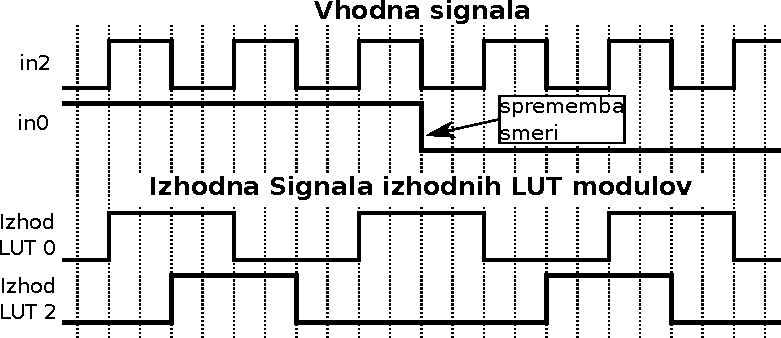
\includegraphics[width=8cm]{obracanje_smeri_potek}}
    \caption{Prikaz izhodnih signalov iz CLB koprocesorja pri simulaciji 
             inkrementalnega dajalnika, glede na simulirane vhodne signale}
    \label{fig:obracanje_smeri}
\end{figure}

Celotna shema končne implementacije je prikazana na sliki
\ref{fig:koncna_shema}.

\begin{figure}[htb]
    \centerline{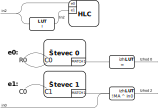
\includegraphics[width=8cm]{koncna_shema}}
    \caption{Shema končne implementacije simuliranega inkrementalnega
             dajalnika z uporabo CLB koprocesorja}
    \label{fig:koncna_shema}
\end{figure}


\section{Vhodni signali v CLB}
vhodni signali v poglavju \ref{sec:nastavitve_podsklopov} so bili za čas
nastavljanja podsklopov zaradi enostavnejšega dela le simulirani. Za delovanje
pa je potrebno signal speljati iz enega od modulov na integriranem vezju. Kot
je razbrati iz poglavja \ref{sec:nastavljanje_clb}, potrebujemo kvadratni
vhodni signal z nastavljivo frekvenco ter signal za obračanje smeri, ki bo v
naravnem stanju prevzel logično 1, ob pritisku pa logično 0.

\subsection{Generiranje kvadratnega signala}
Za vhodni signal v CLB je uporabljen izhod iz ``eCAP'' modula, ki je v osnovi
števec. Ta odločitev je nastala zgolj zaradi 32-bitnega števca v omenjenem
modulu, kar omogoča natančnajšo določitev periode predvsem pri nizkih
frekvencah (najnižja frekvenca = $200 MHz/2^{32} \approx 0,046 Hz$). Modul
preko pulzno-širinske modulacije generira kvadratni signal s polovičnim
delovnim ciklom. Implementacija funkcije za usposobitev ``eCAP'' modula v
načinu ``apwm'' je prikazana na seznamu \ref{lst:ecap_init}.

\begin{lstlisting}[language=C,
                   caption={Implementacija funkcije za usposobitev ``eCAP'' 
                            modula v ``apwm'' načinu},
                   label={lst:ecap_init}]
void ECAP_apwm_init(float freq, float duty)
{
    /* Setup APWM mode on CAP1, */
    /* set period and compare registers */

    /* Enable APWM mode */
    ECap1Regs.ECCTL2.bit.CAP_APWM = 1;
    /* Set Period value */
    ECap1Regs.CAP1 = CPU_FREQ / freq;
    ECap1Regs.CAP3 = CPU_FREQ / freq;
    /* Set Compare value */
    ECap1Regs.CAP2 = ECap1Regs.CAP1 * duty;
    ECap1Regs.CAP4 = ECap1Regs.CAP3 * duty;

    /* Initialize GPIO pins for APWM1. */
    InitAPwm1Gpio();
}
\end{lstlisting}

Opazimo lahko, da je za nastavitev delovanja potrebno določiti le dolžino
periode in primerjalne vrednosti. Slednja je namenjena preklopu iz visokega v
nizko stanje pri generiranju PWM signala. Preko te funkcije tako generiramo
signal z določitvijo frekvence in vklopnega razmerja (``freq'' in ``duty'') Za
boljši vpogled v sistem je preko ``GPIO'' modula ta signal speljan tudi iz
naprave, kjer ga lahko opazujemo z osciloskopom ali logičnim analizatorjem.

Ta signal je nato priključen na lokalni vhod 2 CLB koprocesorja, ter opravlja
vlogo prej simuliranega vhoda ``in2''.

\subsection{Signal za obračanje smeri}
Za obračanje smeri je bil izbran signal ``GPIO24''. Ta je nastavljen kot vhod z
notranjim ``pull-up'' uporom, kar pomeni, da bo v odprtem položaju zavzel
logično 1. Preko vhodnega vodila je priključen na vhod 0 CLB koprocesorja in s
tem prevzema mesto prej simuliranega signala ``in0''.


\section{Delovanje inkrementalnega dajalnika}
Za lažjo uporabo simuliranega inkrementalnega dajalnika so vse nastavitve, ki
niso del orodja ``CLB Tool'' zapakirane v funkciji ``CLB1\_init''. Za končnega
uporabnika pa je vse skupaj razkrito v funkciji, prikazani na seznamu
\ref{lst:klic_enkoderja}

\filbreak
\begin{lstlisting}[language=C,
                   caption={Implementacija funkcije za nastavitev 
                            inkrementalnega dajalnika},
                   label={lst:klic_enkoderja}]
void InitEncoder(float frequency)
{
    /* Initialize ECAP in APWM mode */
    /* with 1/2 duty cycle. */
    ECAP_apwm_init(frequency*2, 0.5);

    /* Initialize the CLB1 block. */
    CLB1_init(CLB1_BASE);
}
\end{lstlisting}

Funkciji nastavimo frekvenco inkrementalnega dajalnika in preko tega se nastavi
``eCAP'' modul z dvokratnikom te frekvence. Ta ima seveda vlogo vhodnega
signala v CLB koprocesor. S seznama \ref{lst:klic_enkoderja} lahko vidimo tudi
klic prej omenjene funkcije ``CLB1\_init'', ki skrbi za nastavitev vseh ostalih
parametrov CLB koprocesorja.


\section{Zaključek}
Iz praktičnega primera lahko razberemo, da je CLB koprocesor uporaben
dodatek za marsikatero aplikacijo, kjer bi z njim lahko nadomestili FPGA čip. V
grobem lahko rečemo, da trditve proizvajalca (ob ignoriranju tržnih
izmišljotink seveda) v veliki meri držijo. CLB lahko marsikje nadomesti FPGA,
je lažji za programiranje, ter je seveda nameščen direktno na samem
integriranem vezju, kar med drugim v veliko primerih pomeni tudi nižjo ceno.

Grafični vmesnik ``CLB Tool'' zaradi svoje narave zahteva veliko
potrpežljivosti. Če je to težava pri tako majhni aplikaciji, si je lahko
predstavljati težavnost pri obsežnih projektih.

Koprocesor pa žari pri majhnih projektih, kjer je bistvenega pomena hitra
implementacija ter se manipulira z manjšim številom signalov. Prav tako je
vsakemu programerju omogočena enostavna uporaba, brez da bi se popolnoma
posvečal takšnim vezjem. Predvsem pa povezave CLB-ja z ostalimi perifernimi
napravami \cite{fpga-to-clb} omogočajo, da se CLB uporabi tudi samo za
razširitev funkcionalnosti periferne naprave (e.g. SPI vodilu lahko dodamo
kompenzacijo zamika signalov med prenosom, združujemo več PWM signalov za
generiranje prižilnih pulzov pri eksotičnih toplogijah močnostne elektronike...


\section{Dodatno branje}
Več informacij o sami implementaciji CLB je opisanih v \cite{clb-designing}. Za
migracijo obstoječih FPGA projektov na CLB in različnih možnostih uporabe
CBL-ja pa je precej dober uvod vir \cite{fpga-to-clb}.


\printbibliography


\end{sloppypar}
\end{document}


